% ****** Start of file apssamp.tex ******
%
%   This file is part of the APS files in the REVTeX 4.1 distribution.
%   Version 4.1r of REVTeX, August 2010
%
%   Copyright (c) 2009, 2010 The American Physical Society.
%
%   See the REVTeX 4 README file for restrictions and more information.
%
% TeX'ing this file requires that you have AMS-LaTeX 2.0 installed
% as well as the rest of the prerequisites for REVTeX 4.1
%
% See the REVTeX 4 README file
% It also requires running BibTeX. The commands are as follows:
%
%  1)  latex apssamp.tex
%  2)  bibtex apssamp
%  3)  latex apssamp.tex
%  4)  latex apssamp.tex
%
\documentclass[%
 reprint,
%superscriptaddress,
%groupedaddress,
%unsortedaddress,
%runinaddress,
%frontmatterverbose, 
%preprint,
%showpacs,preprintnumbers,
%nofootinbib,
%nobibnotes,
%bibnotes,
 amsmath,amssymb,
 aps,
%pra,
%prb,
%rmp,
%prstab,
%prstper,
%floatfix,
]{revtex4-1}

\usepackage{graphicx}% Include figure files
\usepackage{dcolumn}% Align table columns on decimal point
\usepackage{bm}% bold math
\usepackage{color}
%\usepackage{hyperref}% add hypertext capabilities
%\usepackage[mathlines]{lineno}% Enable numbering of text and display math
%\linenumbers\relax % Commence numbering lines

%\usepackage[showframe,%Uncomment any one of the following lines to test 
%%scale=0.7, marginratio={1:1, 2:3}, ignoreall,% default settings
%%text={7in,10in},centering,
%%margin=1.5in,
%%total={6.5in,8.75in}, top=1.2in, left=0.9in, includefoot,
%%height=10in,a5paper,hmargin={3cm,0.8in},
%]{geometry}

%%%%%%%%%%%%%%%%%%%%%%%%%%%%%%%%%%%%%%%%%%%%%%%%%%%%%%%%%%%%%%%%%%%%%
%  needed macros:

%new commands:

%\newcommand{\juan}[1]{\textcolor{blue}{{#1}}}
%\newcommand{\keisuke}[1]{\textcolor{magenta}{#1}}
%\newcommand{\jim}[1]{\textcolor{green}{#1}}
%\newcommand{\todo}[1]{\textcolor{red}{{#1}}}
\newcommand{\juan}[1]{\textcolor{black}{{#1}}}
\newcommand{\keisuke}[1]{\textcolor{black}{#1}}
\newcommand{\jim}[1]{\textcolor{black}{#1}}
\newcommand{\todo}[1]{\textcolor{black}{{#1}}}
%text macros:

\def\etal{{\it et al.}}
\def\etc{{\it etc.}}
\def\eg{{\it e.g.}}
\def\Tab#1{Tab.~\ref{#1}}
\def\Fig#1{Fig.~\ref{#1}}
\def\Figs#1{Figs.~\ref{#1}}
\def\Eq#1{Eq.~(\ref{#1})}
\def\Ref#1{Ref.~\cite{#1}}
\def\Refs#1{Refs.~\cite{#1}}



% math mode macros:

\def\ee{e^+e^-} 

%%%%%%%%%%%%%%%%%%%%%%%%%%%%%%%%%%%%%%%%%%%%%%%%%%%%%%%%%%%%%%%%%%%%%%


\begin{document}

\preprint{LCCPEB---}

\title{The International Linear Collider \\ A Global Project}% Force line breaks with \\
\thanks{Version 1.3}%

\author{Jim Brau}
% \altaffiliation[Also at ]{Physics Department, XYZ University.}%Lines break automatically or can be forced with \\
\author{et.al.}%
 \email{Second.Author@institution.edu}
\affiliation{%
 Authors' institution and/or address\\
% This line break forced with \textbackslash\textbackslash
}%

\collaboration{Linear Collider Collaboration}%\noaffiliation

\date{\today}% It is always \today, today,
             %  but any date may be explicitly specified

\begin{abstract}
Input from the International Linear Collider community for the European Strategy Update 

\end{abstract}

\pacs{Valid PACS appear here}% PACS, the Physics and Astronomy
                             % Classification Scheme.
%\keywords{Suggested keywords}%Use showkeys class option if keyword
%display desired
\maketitle

%\tableofcontents

\section{\label{sec:intro}Introduction}

%\todo{ 1 page - Jim and Juan
% Introduce the ILC250, brief overview of status (technical maturity and TDR, staging, cost analysis, status of political situation) }

\juan{The central issue in particle physics today is the search for new phenomena} needed to address shortcomings of the highly successful Standard Model.  \juan{These new effects can manifest as new particles, new forces or deviations in the predictions of the Standard Model derived from high precision measurements.}
With the discovery of the Higgs boson in 2012 at the Large Hadron Collider,
the Standard Model was completed. 
While theoretically self-consistent, but in the absence of anticipated new physics beyond the Standard Model,
     a number of issues remain unaddressed; the Standard Model is an incomplete theory of the
     fundamental interactions.
%While theoretically self-consistent, with
%no evidence of physics beyond the Standard Model having appeared, a number of issues remain
%unaddressed, leaving the Standard Model as an %incomplete theory of the fundamental
%interactions.  
New particles or forces could advance our understanding
of how the physics of the Standard Model fits into a more complete
picture of the nature of the universe.

\jim{The international Linear Collider (ILC) has the capabilities needed now to address the central physics issues. 
First and most importantly, it provides unprecedented precision 
in the measurements and searches needed to pursue these questions.  
For example, ILC will have unique sensitivity to test the 
Higgs couplings, particularly critical should the deviations 
from the Standard Model be small. It offers a range of 
operating energies, both through beam energy variation 
and straight-forward accelerator energy upgrades.  
The energy upgrades will allow the ILC to remain a powerful 
discovery vehicle for decades. Beam polarizations provide 
unique access to important and powerful physics parameters. 
Finally, and critically, the technology is mature, 
ready for implementation today.}

Among the outstanding questions that are the focus of energy frontier
efforts are the explanation of the apparent mismatch of the scale of
electroweak physics with the Planck scale, or the hierarchy problem.
Why is the Higgs mass as light as it is~?
The Standard Model does not offer any explanation for the evidence for dark matter.
Likewise, gravitation is not included.  These and other issues
motivate intense efforts to \juan{test the consistency} of the Standard Model \juan{to high accuracy}
and \juan{look for} small deviations that would provide clues toward answering such
open questions.

For more than twenty years the worldwide community has been engaged in a research
program developing the technology required to realize a high energy linear collider
to precisely measure electron-positron collisions, contributing to 
answering the critical questions at the energy frontier, such as the hierarchy problem,
the nature of dark matter and even the relationship to gravity.
\jim{In the mid-1990's, as various technology options to realize a high energy linear collider
were emerging, the ICFA-directed Linear Collider Technical Review Committee
developed a standardized way of comparing the  technologies in terms of parameters such as power consumption and luminosity. In 2002, ICFA 
set up a second review, that concluded
both the warm and cold technologies had developed to the point where either would work
for a linear collider.
This led to
the International Technology Review Panel (ITRP), charged by ICFA to recommend an option.  Superconducting radiofrequency (SCRF) was chosen in 2004, in a large part due to its energy efficiency and potential for broader applications.  Many of those applications have been realized bringing the technology to a high level of readiness for the ILC.}
The effort to design and establish the technology for the linear collider 
culminated in the publication of the Technical Design Report (TDR)
for the International Linear Collider (ILC) in 2013~\cite{Behnke:2013xla}. 
\juan{  In its current form, the \jim{ILC250} is a $250\,{\mathrm{GeV}}$ (extendable up to $1\,{\mathrm{TeV}}$) linear $e^+e^-$ collider, based on $1.3\,{\mathrm{GHz}}$ superconducting radio-frequency (SCRF) cavities. It is designed to  achieve a luminosity of $1.5\cdot 10^{34}~{\mathrm{cm}}^{-1}{\mathrm{s}}^{-1}$ and provide an integrated luminosity of $350\,{\mathrm{fb}}^{-1}$ in the first four years of running. The electron beam will be polarised to $80\,\%$, and positrons with $30\,\%$ polarization will be provided if the undulator based positron source concept is employed.} The parameters were set by considerations of the physics goal,
with an energy reach designed to likely provide access to the mechanism of 
electroweak symmetry breaking (Higgs or no-Higgs)~\cite{Baer:2013cma}.


\juan{ The collider design is thus the result of nearly twenty years of R\&D. The heart of the ILC, the superconducting cavities, is based on the pioneering work at the TESLA Test Facility, beginning in the 1990s. Some other aspects emerged from the R\&D carried out for the JLC/GLC and NLC projects, which were based on room-temperature accelerating structures. From 2005 to the publication of the TDR~\cite{Behnke:2013xla} in 2013, the design of the ILC accelerator was conducted as a worldwide international collaboration, the Global Design Effort (GDE), under a mandate from the International Committee for Future Accelerators (ICFA).
Since then, the Linear Collider Collaboration (LCC) has been coordinating the international activities for both the ILC and CLIC projects, again mandated by ICFA.}

%The ILC presented in the TDR is a 200-500 GeV (extendable to 1 TeV) centre-of-mass 
%high luminosity linear electron-positron collider, based on 1.3 GHz superconducting radio-frequency (SCRF)
%accelerating technology~\cite{Adolphsen:2013kya}. 
%Some relevant parameters are given in Tab.~\ref{tab:ilc-params}.}

Once the mass of the Higgs boson was known, it was established that the
linear collider could begin to address these questions in unique fashion
with an initial center-of-mass energy of 250 GeV \jim{at a cost reduced from the TDR.}
A revised design of the ILC (the ILC250) has been presented~\cite{Evans:2017rvt}
based on the ILC TDR.  This design retains the final focus and beam dump
capability to extend the centre-of-mass energy to \juan{higher energies}.  The cost estimate for ILC250 has 
been developed and presented as well.

Additionally, advances in the theoretical understanding of the impact of precision
measurements of the Higgs boson couplings by ILC250 have increased the understanding
of their sensitivity to physics beyond the Standard Model~\cite{Barklow:2017suo,Fujii:2017vwa}. 

The experimental community has developed the designs for two complementary detectors,
ILD and SiD~\cite{Behnke:2013lya}.  These detectors are designed to optimally address the
ILC physics goals.  They are based on a detector R\&D program that has \juan{as well}
contributed a number of advances in detector capabilities \juan{and applications beyond the ILC}.
An additional key need for the experimental program is the software and computing.

This report summarizes the current status of this effort \juan{describing the physics reach, the technological maturity of the accelerator, detector and software/computing development plus a short discussion on the possible future scenarios to realize the project.} 

\section{\label{sec:phys}Physics}

The physics case for the construction of the ILC is very strong.   The
most important item in this case is the ability to study the couplings
of the Higgs boson with high precision.  The ILC at 250~GeV also
presents many opportunities to discover new particles that go beyond
the capabilities of the LHC.  Finally, the ILC at 250~GeV opens the
door to further exploration of $\ee$ reactions at higher energies. 
The ILC physics case is reviewed at greater length in the reference
document~\cite{ILCforESS}. 

The Higgs boson is a necessary yet also mysterious part of the
Standard Model of Particle Physics (SM).    In the SM, the Higgs field
couples to every elementary particle and provides the mass for all
quarks, leptons, and heavy vector bosons.   The LHC has now discovered
the Higgs particle and confirmed the presence of the couplings responsible for the
masses of the $W$, $Z$, $t$, $b$, and $\tau$~\cite{LHCHiggssummary}. 
 However, many mysteries are still
buried here.   The Higgs couplings are not universal, as the gauge
couplings are, and their pattern (which is also the pattern of lepton
and quark masses) is not explained by the SM.  The basic phenomenon that provides
mass for elementary particles---the spontaneous breaking of the gauge
symmetry $SU(2)\times U(1)$---is not explained, and actually cannot be
explained, by the SM.   The Higgs boson could also couple to new
particles and fields that have no SM gauge interactions and are
otherwise completely inaccessible to observation.  Thus, detailed
examination of the Higgs boson properties should be the next major
goal for particle physics experiements.

Within the SM, the couplings of the Higgs boson are specified now that
the parameters of the model, including the Higgs boson mass, are
known.  Expected improvements in the SM parameters in the 2020's will
allow these couplings to be predicted to the part-per-mille level~\cite{Lepage:2014fla}.
Models of new physics correct  these predictions.   These corrections
are predicted to be small, at the 10\% level or below, but they can
be visible to precision experiments.   Most importantly, different
classes of models affect the various Higgs couplings differently, so that
systematic measurement of the Higgs couplings can reveal clues to the
nature of the new intereractions.   The precision study of the Higgs
boson interactions then provides a new method both to {\it discover}  the
presence of physics beyond the SM and to {\it learn}  about its nature.

The couplings of the Higgs boson are now being studied at the LHC.
The LHC experiments have made remarkable progress in measuring the
couplings and the Higgs boson, and they expect impressive further progress, as
documented in the HL-LHC Yellow Report~\cite{Yellow}.  The uncertainty
projections
from the Yellow Report   are shown in Fig.~\ref{fig:ILCLHC}.   These
measurements are very challenging.   Aside from events in
which the Higgs boson appears as a narrow resonance (the decays to
$\gamma\gamma$ and $4\ell$), Higgs boson events are not visibly
distinct from SM background events.  Analyses start from
signal/background ratios of about  1/10  (better for VBF production,
but 
worse for $Vh$ production with $h\to b\bar b$) and then apply strong
selections to make the Higgs signal visible.   To reach the
performance levels predicted in  the Yellow Report, it is necessary to
determine the level of suppression of SM backgrounds to better than
 1\% accuracy.  At
the same time, these projected uncertainties do not allow the LHC experiments to
observe, for example, an anomaly of 5\% in the $hWW$ coupling to
3$\sigma$ significance.   To prove the presence of such small
deviations, which are typical in new physics models, we need to take a
different approach. 

What is needed for a precision Higgs boson measurement program
is a new experimental method in which all individual Higgs boson decay events
are manifest
and can be studied in detail.   This is provided by the reaction
$\ee\to Zh$ at 250~GeV in the center of mass.
  With small and precisely calculable SM backgrounds, any $Z$ boson
  observed with a lab energy of 110~GeV is recoiling against a Higgs
  boson.  By selecting such events, we learn the complete profile of Higgs boson
  decays, to SM leptonic and hadron modes and even to invisible or
  partially visible exotic modes. 

Further, since the cross section for Higgs production can be measured
without measuring any property of the Higgs boson, the scale of Higgs
couplings can be determined and the individual couplings can be
absolutely normalized.  Each individual coupling can be compared to
its SM prediction.

In the description of new physics by an  $SU(2)\times U(1)$-invariant
effective field theory (EFT), new physics effects on the  Higgs boson
couplings to $W$ and $Z$ are related to new physics effects on
precision electroweak observables and in $\ee\to W^+W^-$.   This
latter reaction can also be studied with high precision at an $\ee$
collider.  Beam polarization at the ILC is at especially powerful tool
to separate the contributions of different EFT
coefficients.  We can also make use of  measurements such as the 
ratio of branching ratios  $BR(h\to \gamma\gamma)/BR(h\to ZZ^*)$ that
will be obtained directly at the HL-LHC. 
  In \cite{Barklow:2017suo}, it is shown that {\it all}
relevant EFT
coefficients can be fit {\it simultaneously} from the multiple
observables available in this approach, giving a 
determination of Higgs boson couplings that is as
model-independent as the underlying EFT description itself. 
 This analysis is reviewed in detail in
\cite{ILCforESS}. 
For the nominal ILC program at 250~GeV, we predict that the Higgs
coupling to $b$ quarks will be measured to 1.1\% accuracy and the
couplings to $W$ and $Z$ to 0.7\% accuracy.  The full set  of  expected
uncertainties  is shown in Fig.~\ref{fig:ILCmodelindep}.    The 
discovery of any anomaly at 250~GeV can be confirmed in running at
500~GeV 
using additional reactions  such as $WW$ fusion production of the
Higgs boson.   Measurements at this
level can discover---and distinguish---models of new physics over a
wide space of possibilities, even for models in which the predicted new
particles are too heavy to be discovered at the
LHC~\cite{Barklow:2017suo}.

Figure~\ref{fig:ILCLHC} compares the ILC projections to those in the
HL-LHC Yellow Report~\cite{Yellow}.   The LHC projections include
model-dependent assumptions.  To assist the comparison, we have imposed
these assumptions also in the ILC analysis.   The details of these  ILC
projections are presented in \cite{ILCforESS}. 

%%%%%%%%%%%%%%%%
\begin{figure}
\begin{center}
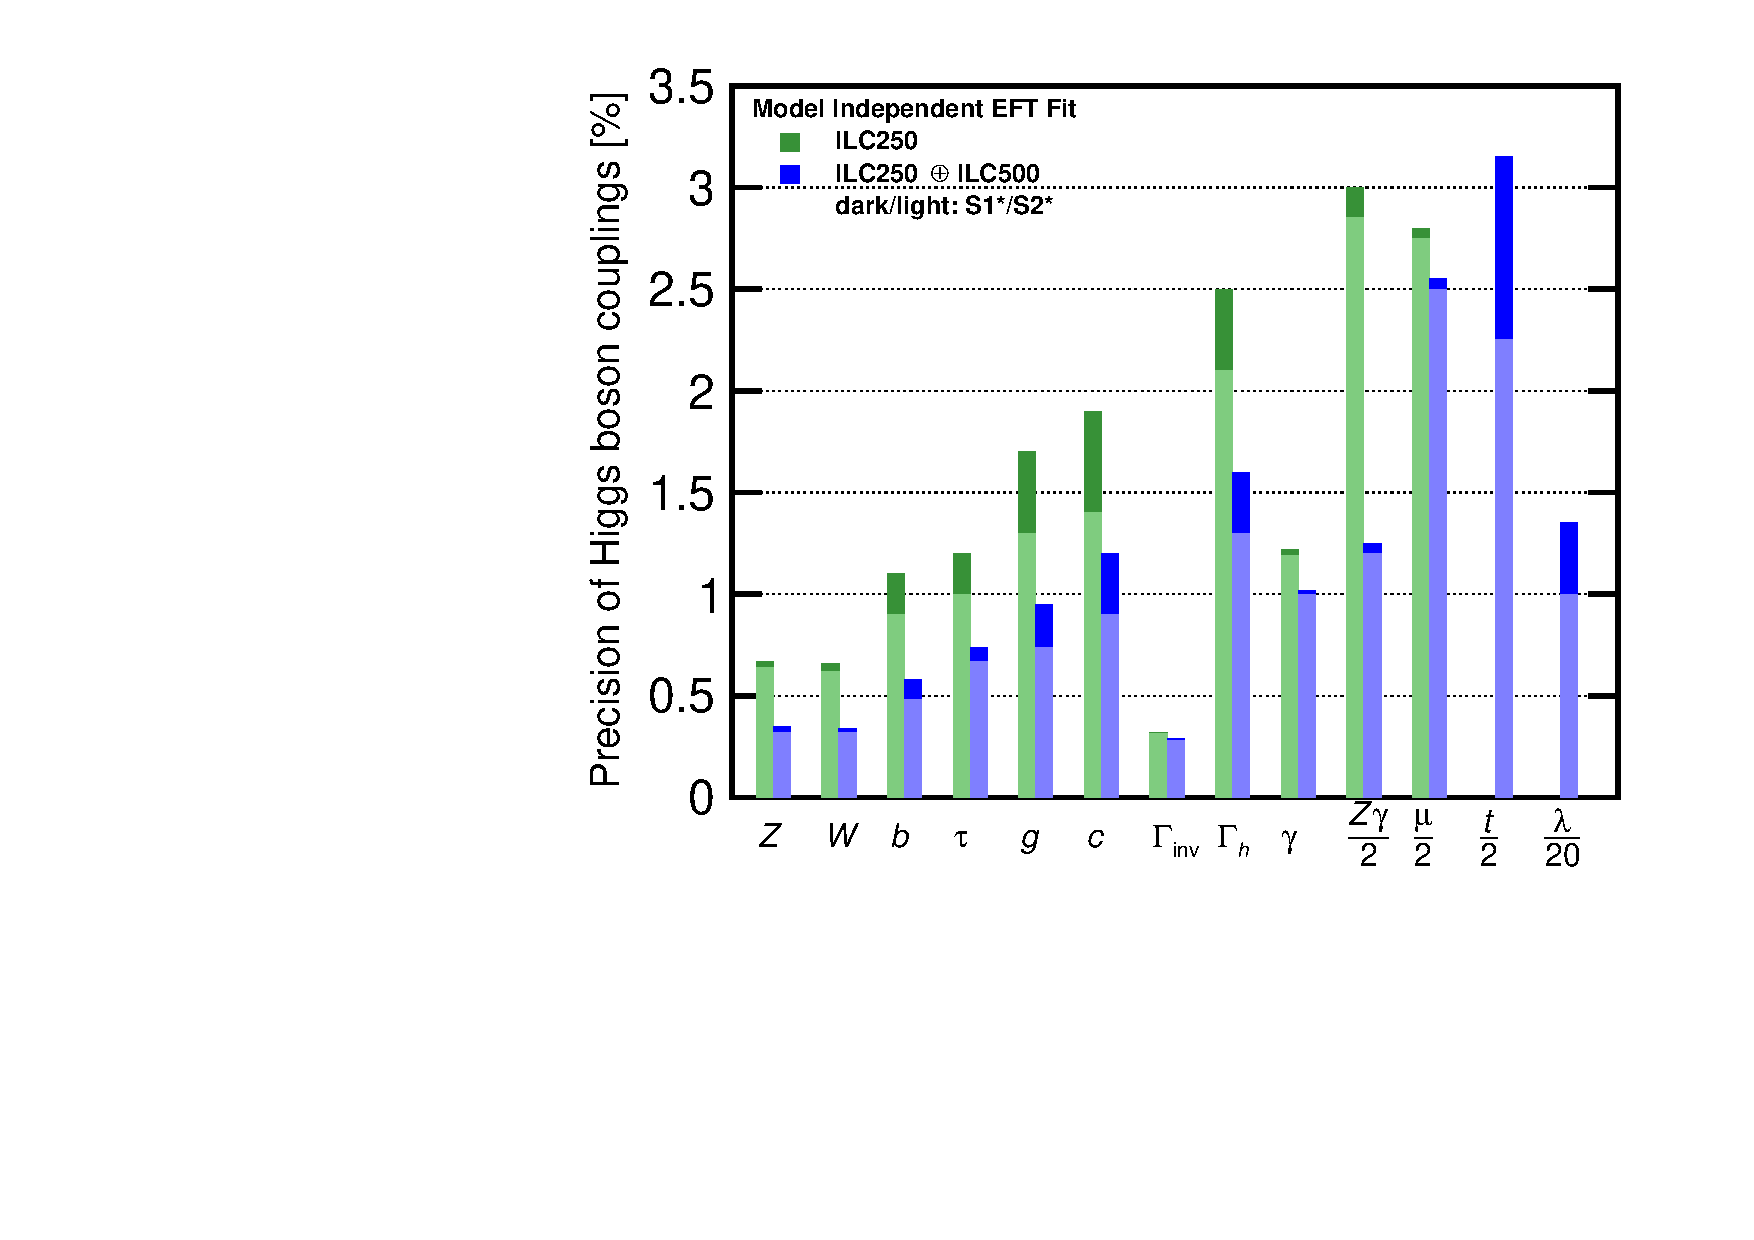
\includegraphics[width=0.70\hsize]{figures/ModelindepSummary.pdf}
\caption{Projected Higgs boson coupling uncertainties for the ILC
  program at 250~GeV and an energy upgrade to 500~GeV, using the
  highly model-independent analysis presented in \cite{Barklow:2017suo}. This
  analysis makes use of  data on $\ee\to W^+W^-$ in addition to Higgs
  boson observables and also incorporates projected LHC results, as described
  in the text. }
\label{fig:ILCmodelindep}
\end{center}
\end{figure}
%%%%%%%%%%%%%%%%%%%%%%%%%%%%%%%%%%%%%%%%%%%%%%%%%%%%%%%%%%%%%%
%%%%%%%%%%%%%%%%
\begin{figure}
\begin{center}
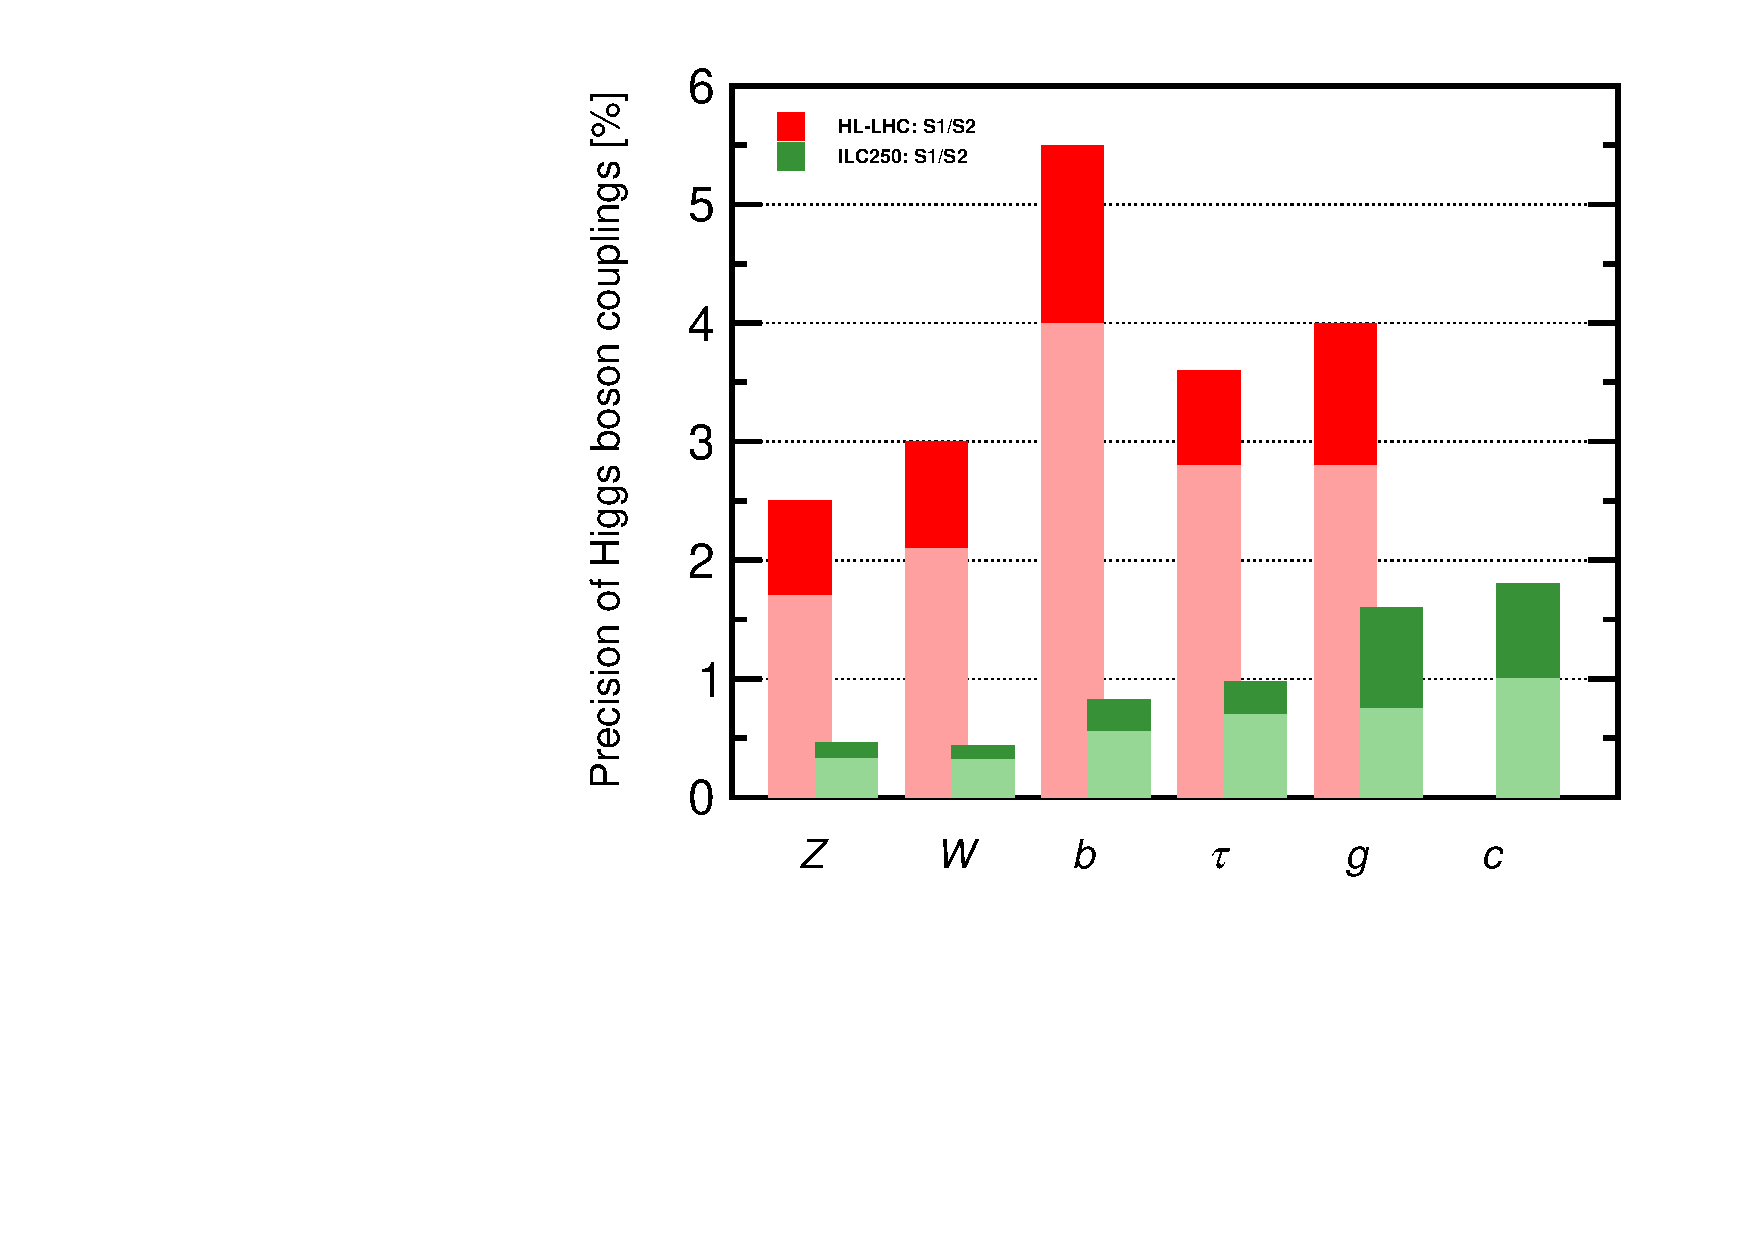
\includegraphics[width=0.70\hsize]{figures/ModeldepSummary.pdf}
\caption{Projected Higgs boson coupling uncertainties for the LHC and
  ILC
using the model-dependent assumptions appropriate to the LHC Higgs
coupling fit.   The
dark and light red bars represent the projections in the scenarios S1
and S2 presented in  \cite{Yellow}.  The scenario S1 refers to
analyses with our current understanding; the scenario S2 refers to
more optimistic assumptions in which experimental errors decrease with
experience.  The dark and light green bars represent the
projections in the ILC scenarios in similar S1 and S2 scenarios defined in
\cite{ILCforESS}. 
 The dark and light blue bars show the projections for scenarios S1 and S2
when
data from the 500~GeV run of the ILC is included.}
 \label{fig:ILCLHC}
\end{center}
\end{figure}
%%%%%%%%%%%%%%%%%%%%%%%%%%%%%%%%%%%%%%%%%%%%%%%%%%%%%%%%%%%%%%


In addition to decays predicted in the SM, the Higgs boson could decay
to particles with no SM gauge interactions.    These decays may
include invisible decays (\eg, to a pair of dark matter particles $\chi$)  or
partially invisible decays (\eg, to $b\bar b \chi \chi$).   The ILC
can robustly seach for all types of exotic decays  to the 
part-per-mille level of branching ratios~\cite{Liu:2016zki}.

The ILC can also search for particles produced through electroweak
interactions, closing gaps that are left by searches at the LHC.  An
important example is the Higgsino of supersymmetric models.   If the
mass  differences among Higgsinos is smaller than a few GeV---which is
actually the prediction of currently allowed models---then Higgsinos
of 100~GeV mass would be produced copiously at the LHC, but this
production would not be registered by LHC triggers.  In the clean
environment 
of the ILC, even such fragile signatures as this 
would be discovered and the new particles 
studied with percent-level precision~\cite{Higgsino}.

 ILC precision
measurements of $\ee\to f\bar f$ processes at 250~GeV have a sensitivity to new
electroweak gauge bosons comparable to (and complementary with) 
direct searches at the LHC.  The reaction $\ee\to b\bar b$ is
particularly interesting, since models of the top quark mass with
composite Higgs bosons can give significant corrections in this
reaction~\cite{eetobb1,eetobb2}.

The ILC at 250~GeV can be the first step to the study of $\ee$
reactions at higher energy.   A linear $\ee$ collider is extendable in
energy by making the accelerator longer or by improving the
acceleration gradient. Extensions to 500~GeV and 1~TeV were envisioned
in ILC Technical Design Report~\cite{Behnke:2013xla}.    These would offer a
measurement of the top quark mass to 40~MeV, measurements of the top
quark electroweak couplings to the per-mille level, measurement of the
Higgs coupling to the top quark to 2\% accuracy, and measurement of
the triple Higgs boson coupling to 10\%  accuracy. They  also would be
the setting for much 
deeper searches for new particles with electroweak interactions.
A higher-gradient accelerator in the ILC tunnel could reach even
higher energies.  The
ILC promises a long future beyond its initial 250~GeV stage.





\section{\label{sec:collider}Collider}

%\todo{ 2 pages - Benno, Shin
%Summary of the ILC250 design (important to note the elements that are retained in first stage to accommodate future energy extensions) }



\juan{The ILC is a $250\,{\mathrm{GeV}}$ (extendable up to $1\,{\mathrm{TeV}}$) linear $e^+e^-$ collider, based on $1.3\,{\mathrm{GHz}}$ superconducting radio-frequency (SCRF) cavities.}

\begin{table}
\begin{tabular}{lccccc}
Quantity & Symbol & Unit & Initial &  \multicolumn{2}{c}{Upgrades} \\
\hline
Centre of mass energy & $\sqrt{s}$ & ${\mathrm{GeV}}$ & $250$ & $500$ & $1000$ \\
Luminosity & \multicolumn{2}{c}{${\mathcal{L}}$ $(10^{34}{\mathrm{cm^{-2}s^{-1}}}$})& $1.35$ & $1.8$ & $4.9$ \\
Repetition frequency &$f_{\mathrm{rep}}$ & ${\mathrm{Hz}}$  & $5$ & $5$ & $4$ \\
Bunches per pulse  &$n_{\mathrm{bunch}}$ & 1  & $1312$ & $1312$ & $2450$ \\
Bunch population  &$N_{\mathrm{e}}$ & $10^{10}$ &$2$ & $2$ & $1.74$ \\
Linac bunch interval & $\Delta t_{\mathrm{b}}$ & ${\mathrm{ns}}$ & $554$ & $554$ & $366$ \\
Beam current in pulse & $I_{\mathrm{pulse}}$ & ${\mathrm{mA}}$& $5.8$ & $5.8$ & $7.6$  \\
Beam pulse duration  & $t_{\mathrm{pulse}}$ & ${\mathrm{\mu s}}$ &$727$ & $727$ & $897$ \\
Average beam power  & $P_{\mathrm{ave}}$   & ${\mathrm{MW}}$ & $5.3$   &$10.5$  & $27.2$ \\  
Norm. hor. emitt. at IP & $\gamma\epsilon_{\mathrm{x}}$ & ${\mathrm{\mu m}}$& $5$ & $10$ & $10$  \\ 
Norm. vert. emitt. at IP & $\gamma\epsilon_{\mathrm{y}}$ & ${\mathrm{nm}}$ & $35$ & $35$ & $35$ \\ 
RMS hor. beam size at IP  & $\sigma^*_{\mathrm{x}}$ & ${\mathrm{nm}}$  & $516$ & $474$ & $335$ \\
RMS vert. beam size at IP &$\sigma^*_{\mathrm{y}}$ & ${\mathrm{nm}}$ & $7.7$  & $5.9$ & $2.7$ \\
Site AC power  & $P_{\mathrm{site}}$ &  ${\mathrm{MW}}$ & $129$ & $163$ & $300$ \\
Site length & $L_{\mathrm{site}}$ &  ${\mathrm{km}}$ & $20.5$ & $31$ & $40$ \\
\end{tabular}
\caption{Summary table of the ILC accelerator parameters in the initial $250\,{\mathrm{GeV}}$ staged configuration
and possible upgrades.
\label{tab:ilc-params}}
\end{table}

The fundamental goal of the design of the ILC is to fulfill the physics objectives outlined in this document in terms of energy and luminosity with a high energy efficiency.
This limits the overall power consumption of the accelerator complex during operation to $129\,{\mathrm{MW}}$ at  $250\,{\mathrm{GeV}}$ and $300\,{\mathrm{MW}}$ at  $1\,{\mathrm{TeV}}$, which is comparable to the power consumption of CERN.
% Stapnes at ALCW2018: 1.35TWh in 2012 -> 154MW on average in 2012
This is achieved by the use of SCRF technology for the main accelerator, which offers a high RF-to-beam efficiency through the use of superconducting cavities, operating at $1.3\,{\mathrm{GHz}}$, where high-efficiency klystrons are commercially available.
At accelerating gradients of $31.5$ to $35\,{\mathrm{MV/m}}$ this technology offers high overall efficiency and reasonable investment costs, even considering the cryogenic infrastructure needed for the operation at $2\,{\mathrm{K}}$. \juan{Some relevant parameters are given in \Tab{tab:ilc-params}.}

The underlying TESLA technology is mature, with a broad industrial base throughout the world, and is in use at a number of free electron laser facilities that are in operation (European XFEL at DESY, Hamburg), under construction (LCLS-II at SLAC, Stanford) or in preparation (SHINE in Shanghai) in the three regions Asia, Americas, and Europe that have contributed to the ILC design. In preparation for the ILC, Japan and the U.S.\ have founded a collaboration for further cost optimisation of the TESLA technology.
In recent years, new surface treatments during the cavity preparation process, such as the so-called nitrogen infusion, have been developed at Fermilab and elsewhere.
They offer the prospect to achieve higher gradients and lower loss rates, even at a less expensive surface preparation scheme than assumed in the TDR, which would lead to a further cost reduction over the current estimate.

When the Higgs was discovered in 2012 and the Japan Association of High Energy Physicists (JAHEP) made a proposal to host the ILC in Japan,
the Japanese ILC Strategy Council conducted a survey of possible sites for the ILC in Japan, looking for  suitable geological conditions for a tunnel up to $50\,{\mathrm{km}}$ in length (as required for a $1\,{\mathrm{TeV}}$  machine), and the possibility to establish a laboratory where several thousand international scientists can work and live. 
As a result, the candidate site in the Kitakami region in northern Japan, close to the larger cities of Sendai and Morioka, was found to be the best option. 
The site offers a large, uniform granite formation, with no active seismic faults, that is well suited for tunneling.
Even at the great Tohoku earthquake in 2011 underground installations in this rock formation were essentially unaffected, which underlines the suitability of this candidate site. 

\Fig{fig_ilc-schematic} shows a schematic overview over the accelerator with its main subsystems.
The accelerator extends over $20.5\,{\mathrm{km}}$, with two main arms that are dominated by the electron and positron main linacs, respectively, at an $14\,{\mathrm{mrad}}$ crossing angle.

 \begin{figure*}[tb]
 %\epsfysize=9.0cm
 \begin{center}
 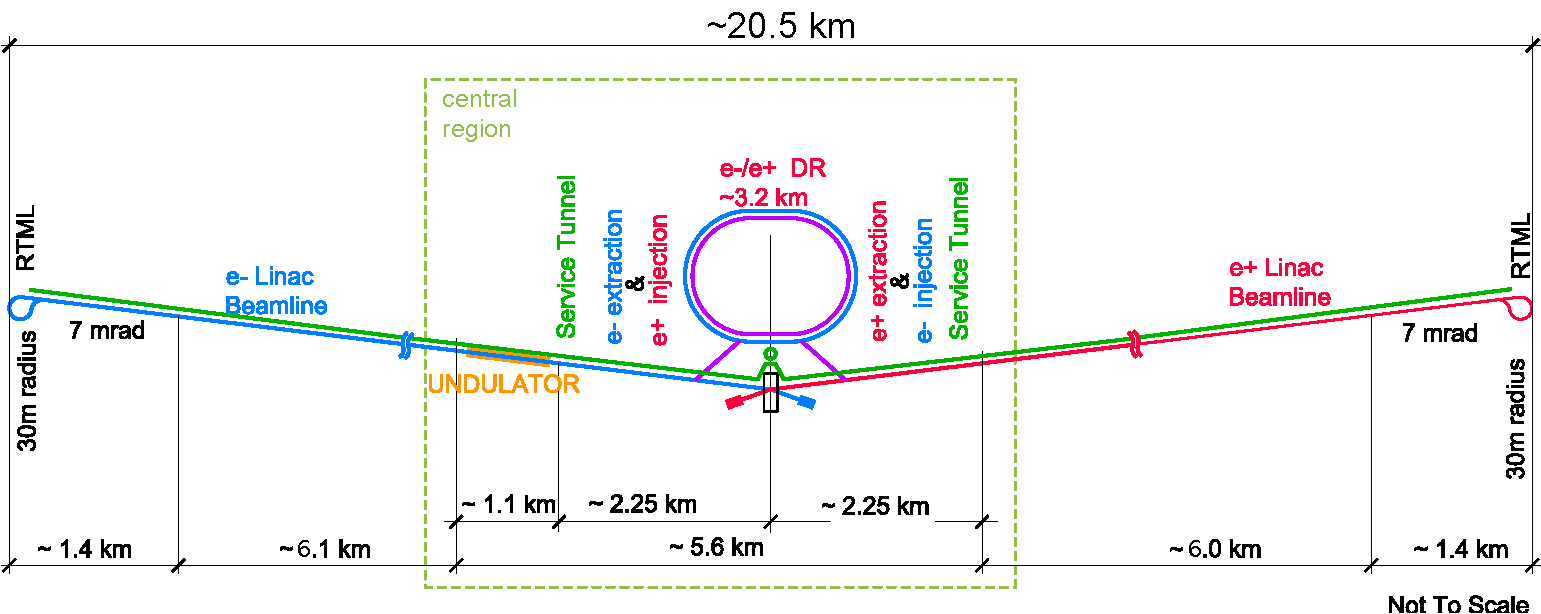
\includegraphics[width=\hsize]{figures/TDR-machine-layout-cartoon-staged.pdf}
\caption{Schematic layout of the ILC in the $250\,{\mathrm{GeV}}$ staged configuration.
\label{fig_ilc-schematic}}
 \end{center}
 \end{figure*}

Electrons are produced by a polarised electron gun located in the tunnel of the positron beam delivery system. A Ti:sapphire laser impinges on a photocathode with a strained GaAs/GaAsP superlattice structure, which will provide  $90\,\%$, electron polarisation at the source, resulting in $80\,\%$ polarisation at the interaction point. The design is based on the electron source of the SLAC accelerator. 

Two concepts for positron production are considered:

The baseline solution employs superconducting helical undulators at the end of the electron main linac, producing polarised photons that are converted to positrons with a $30\,\%$ longitudinal polarisation in a rotating target.
This positron production scheme requires an operational electron linac delivering a beam close to its nominal energy of $125\,{\mathrm{GeV}}$, which is a complication for commissioning and operation. 
%The main technical challenges of this concept are the target and the photon dump. 
%In addition, the undulator photon flux rapidly falls for electron energies below $125\,{\mathrm{GeV}}$, which is a concern for commissioning and operation.  
An alternative design, the electron driven source, utilises a dedicated S-band electron accelerator to provide a $3\,{\mathrm{GeV}}$ beam that is used to produce positrons by pair production.
% on a rotating titanium target. 
%Electrons are produced over a timespan of $66\,{\mathrm{ms}}$, reducing the target heat load and the necessary rotation speed.
%Technical challenges for this concept are radiation in the capture device and beam loading in the first accelerating cavities. 
This source would not provide positron polarisation,
but would have advantages for operation at lower electron beam energies and during commissioning.
% as its operation is independent  from the main linac electron beam, operation at lower electron beam energies is possible and commissioning can begin in parallel to electron source commissioning.
Both concepts are
likely to prove viable when the requisite engineering effort can be devoted to their design.
The current accelerator design is compatible with either option. 
A decision between the alternatives will be made before commencement of the detailed engineering design, based on their relative physics potential, costs, and technical maturity.

Electrons and positrons are injected at $5\,{\mathrm{GeV}}$ into the centrally placed $3.2\,{\mathrm{km}}$ long damping ring complex, where their emittance is reduced to $2\,{\mathrm{pm}}$ ($5\,{\mathrm{\mu m}}$) in the horizontal (vertical) plane within $100\,{\mathrm{ms}}$. 
These emittance numbers are well in line with the performance of today's storage rings for advanced light sources.
To achieve the necessary damping time constant, the damping ring is equipped with $54$ superconducting wigglers. 

The damped beams are transported to the beginning of the main accelerator by two low emittance beam transport lines. Two bunch compressor stages at $5$ and $15\,{\mathrm{GeV}}$ reduce the longitudinal bunch length to $300\,{\mathrm{\mu m}}$ before the beams are accelerated to $125\,{\mathrm{GeV}}$ in the two main linacs.

The main linacs accelerate the beams in superconducting cavities made of niobium, operating at $1.3\,{\mathrm{GHz}}$ frequency and a temperature of $2.0\,{\mathrm{K}}$. 
Each cavity has $9$ cells and is $1.25\,{\mathrm{m}}$ long. The mean accelerating gradient will be $31.5$ to $35\,{\mathrm{MV/m}}$.
Cavities are mounted in $12\,{\mathrm{m}}$ long cryomodules that house $9$ cavities or $8$ cavities plus a quadrupole unit for beam focusing. 
The cryomodules provide cooling and thermal shielding to the cavities and contain all necessary pipes for fluid and gaseous helium at various temperatures, so that no separate helium transport line is necessary.
Cryomodules of this type have been in continuous operation since 2000 in the TESLA Test Facility (TTF, now FLASH) at DESY,  proving their long-term stability. 
Since September 2017, the European X-FEL at DESY has been in operation, utilizing 97 of these cryo modules. 
Cost and performance estimates for the ILC cryomodules are based on the experience from these facilities, and thus can be regarded with high confidence. 

The radiofrequency (RF) power for the cavities is generated by commercially available $10\,{\mathrm{MW}}$ klystrons with an efficiency of $65\,\%$. 
The pulse modulators will be use a new, modular and cost-effective semiconductor design \jim{developed} at SLAC, the MARX modulator.

The cryogenic system design foresees six cryo plants for the main linacs with a size similar to the plants that are operational at CERN (8 plants for the LHC), DESY (for HERA / XFEL) and Fermilab (for the Tevatron); 
two smaller plants would supply the central region including the preaccelerators of the sources and the damping rings. 

Finally, the beam delivery system focuses the beams to the required size of $516\,{\mathrm{\mu m}} \times 7.7\,{\mathrm{nm}} $. 
A feedback system, which profits from the relatively long inter bunch separation of $554\,{\mathrm{ns}}$, ensures the necessary beam stability. 
The necessary nano-beam technology has been tested at the Accelerator Test Facility 2 (ATF-2) at KEK, where beam sizes within $10\,\%$ of the goal for ILC~\footnote{A $41\,{\mathrm{nm}}$ beam size was achieved at TF2, which corresponds to the ILC design goal after scaling for the different beam energies.} have been demonstrated, as well as the feedback system.

The TDR baseline design was for a centre-of-mass energy of $\sqrt{s}=500\,{\mathrm{GeV}}$, upgradeable to a final energy of $1\,{\mathrm{TeV}}$.
After the discovery of the Higgs boson in 2012, interest grew for an accelerator operating as a ``Higgs factory'' at $\sqrt{s}=250\,{\mathrm{GeV}}$, slightly above the maximum for $Zh$ production. 
The design for a $250\,{\mathrm{GeV}}$ version of the ILC has recently been presented in a  staging report by the LCC directorate~\cite{Evans:2017rvt} and was endorsed by ICFA.

This staged version of the ILC  
% (in the preferred ``option A'') 
would have two main linac tunnels about half the length ($6$ instead of $11\, {\mathrm{km}}$) of the $500\,{\mathrm{GeV}}$ TDR design. 
Other systems, in particular the beam delivery system and the main dumps, would retain the dimensions of the TDR design.
Thus, the ILC250 could be upgraded to energies of $500\,{\mathrm{GeV}}$ or even $1\,{\mathrm{TeV}}$ with a reasonable effort, without extensive modifications to the central region. 
Recent studies of rock vibrations from tunnel excavation in a similar geology indicate that the necessary additional main linac tunnels could be largely constructed during ILC operation, so that an energy upgrade could be realised with an interruption in data taking of a couple of years only, compatible with a smooth continuation of the physics programme.

Another upgrade option, which could come before or after an energy upgrade, is a luminosity upgrade. 
Doubling the luminosity by doubling number of bunches per pulse to $2625$ at a reduced bunch separation of $366\,{\mathrm{ns}}$ would require $50\,\%$ more klystrons and modulators and an increased cryogenic capacity. 
The damping rings would also permit an increase of the pulse repetition rate from $5$ to $10\,{\mathrm{Hz}}$. 
This would require a significant increase in cryogenic capacity, or running at a reduced gradient after an energy upgrade.
% Both paths to a luminosity increase would pose large  stress for the positron source target and probably require its redesign, which would be a significant engineering challenge, but not a cost driver.
The projections for the physics potential of the ILC250 are based on a total integrated luminosity of $2\,{\mathrm{ab}}^{-1}$, which assumes at least one luminosity upgrade.

The total project cost for the construction of the $250\,{\mathrm{GeV}}$ accelerator is estimated to be $5,260\,{\mathrm{MILCU}}$ plus $17\,{\mathrm{Mh}}$ of work, where an ILCU (ILC Currency Unit) is defined as $1\,{\mathrm{US\$}}$ in 2012 terms. 
These numbers include the cost for civil engineering and the laboratory, while costs for land acquisition are exempt, as are R\&D costs before the construction start, and costs for the detectors.
The \juan{cost is calculated} as an estimate of the median project cost, without contingency or management reserve.
The cost premium to cover the project cost with $85\,\%$ instead of $50\,\%$ confidence level (loosely speaking, the $1\,\sigma$ uncertainty of the cost estimate) has been estimated to be $23\,\%$ of the estimated cost.

The construction of the accelerator will require nine years after ground breaking, preceded by a four year preparation phase.




\section{\label{sec:detect} Detectors}

%\todo{ 2 pages - Ties, Andy}

%\todo{introductory paragraph is needed to connect with the R\&D section and giving continuity to the whole programme: detector designed being the consequence of the Machine conditions, physics requirements and detector R\&D progress.}

The detector concepts proposed for the ILC have been developed over the past 15 years in a strong international effort. They reflect the requirements placed on the detectors from the science, and have folded in the constraints from the design of the machine, in particular the interaction region, and the results from the R\& D effort which has been described above.  
The main boundary conditions are: 
\begin{figure}[tb]
 %\epsfysize=9.0cm
 \begin{center}
 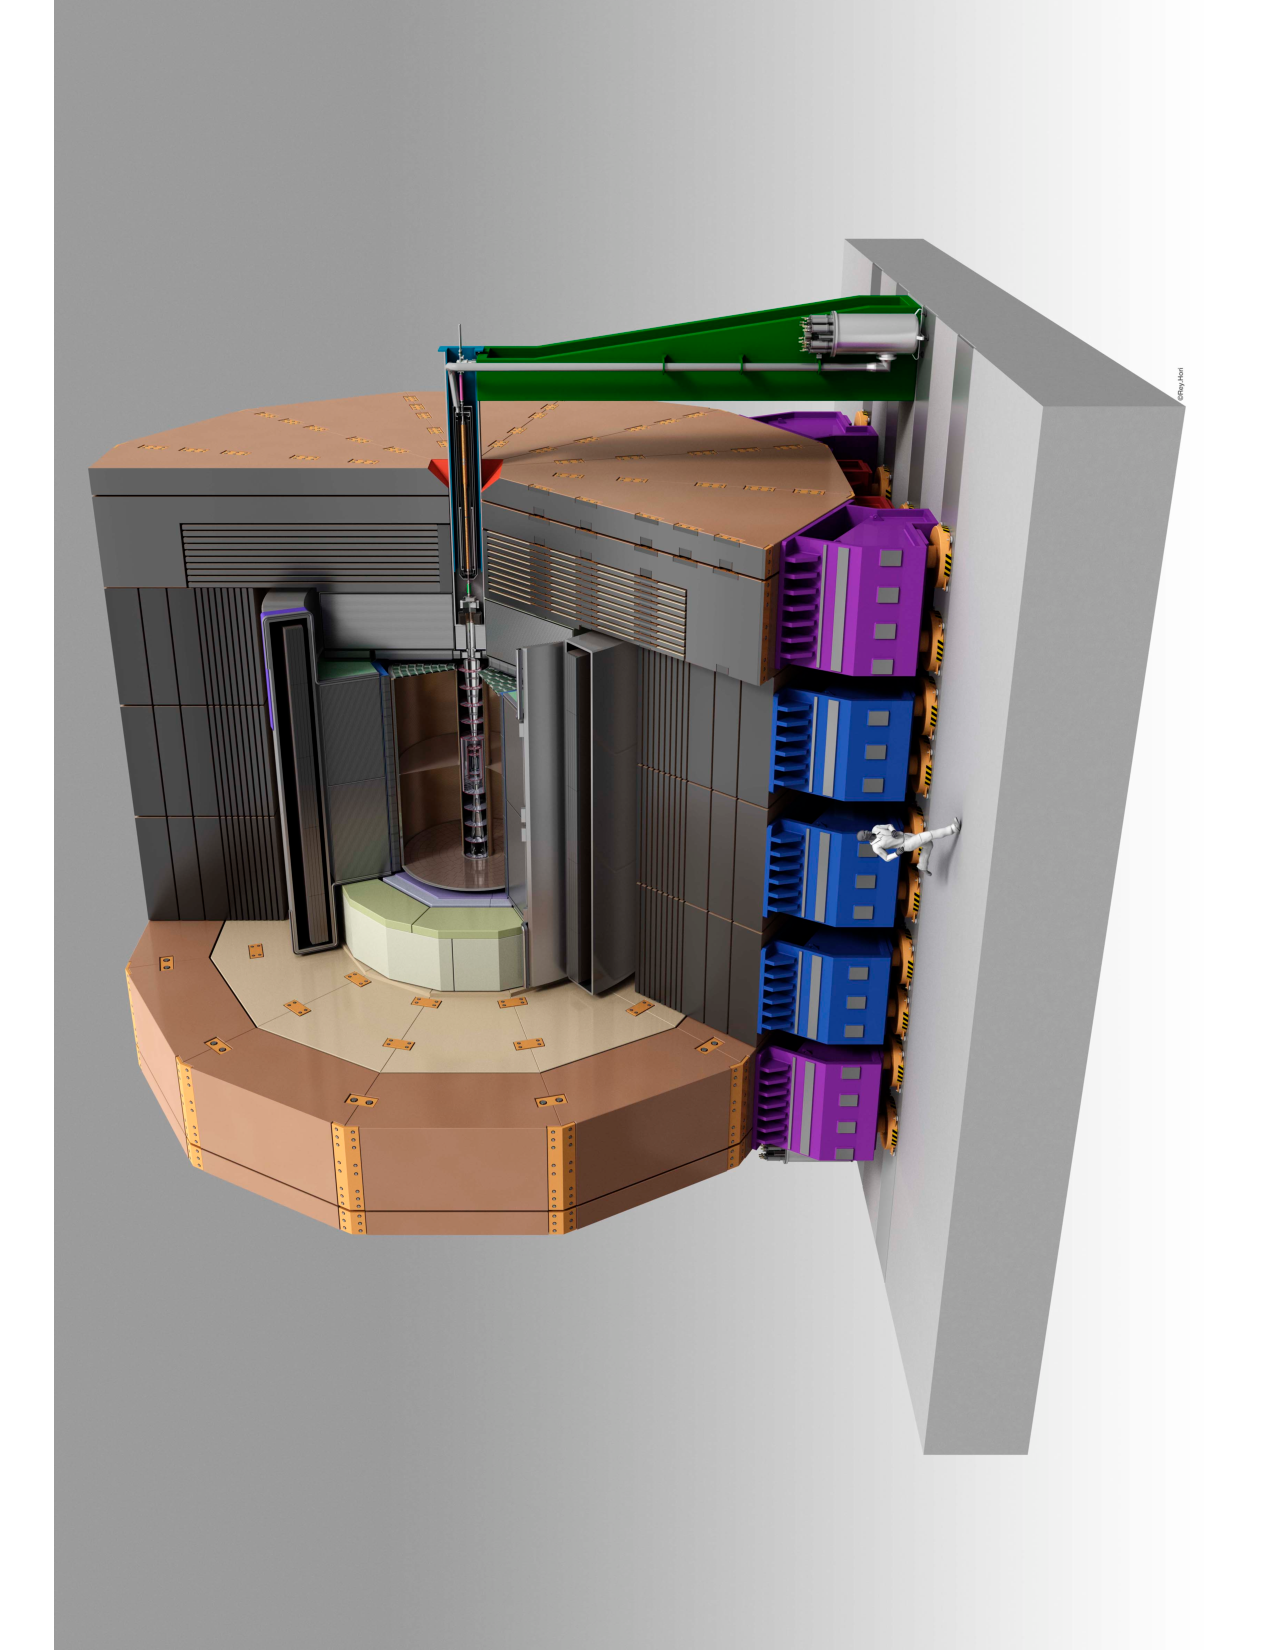
\includegraphics[width=0.8\hsize,angle=-90]{figures/ILD.pdf}
\caption{The ILD detector concept.
\label{fig_ild}}
 \end{center}
 \end{figure}
 
 
\begin{itemize}
 \item The detector has to have an excellent track momentum
   resolution. The benchmark reaction here is the analysis 
of the di-lepton mass in the process $HZ \to H \ell^+
\ell^-$. This reaction allows the reconstruction of the 
Higgs mass independent of its decay mode via the 
reconstruction of the lepton recoil spectrum. In order that 
the momentum resolution of the detector does not limit 
the mass resolution achievable for the recoiling lepton 
system, stringent momentum resolution requirements have to be met. 
\item The reconstruction of the flavour of the final state can 
often be done best with the help of lifetime information of the 
decaying particles. For this, very powerful vertex detectors 
are needed. This is particularly important 
in the Higgs sector, where -- at least for light Higgs bosons -- 
a large fraction of the Higgs decays has bottom 
quarks in the final state. Many other physics signatures will 
produce complex final states with bottom or charm quarks as well. 
A supreme vertex detector therefore is needed to reconstruct these 
long lived particles with excellent resolution. 
\item The overall event is best reconstructed with the 
particle flow measurement. The particle flow technique combines 
the information from the tracking systems and from the 
calorimetric systems in an attempt to reconstruct the 
energy and the direction of all charged and 
neutral particles in the event. To minimize overlaps between 
neighboring particles, and to maximize the probability to 
correctly combine tracking and calorimeter information, 
excellent calorimeters are needed with very high granularity. 
\item Many physics signatures predict some undetectable particles, 
which escape from the detector. They can only be reconstructed by 
measuring the missing energy in the event. This requires 
that the detector is as hermetic as possible, to 
minimize the amount of energy that can escape detection. 
Particular care has to be given to the region surrounding the 
beampipe in the forward direction. 
\end{itemize}

\begin{figure}[tb]
 %\epsfysize=9.0cm
 \begin{center}
 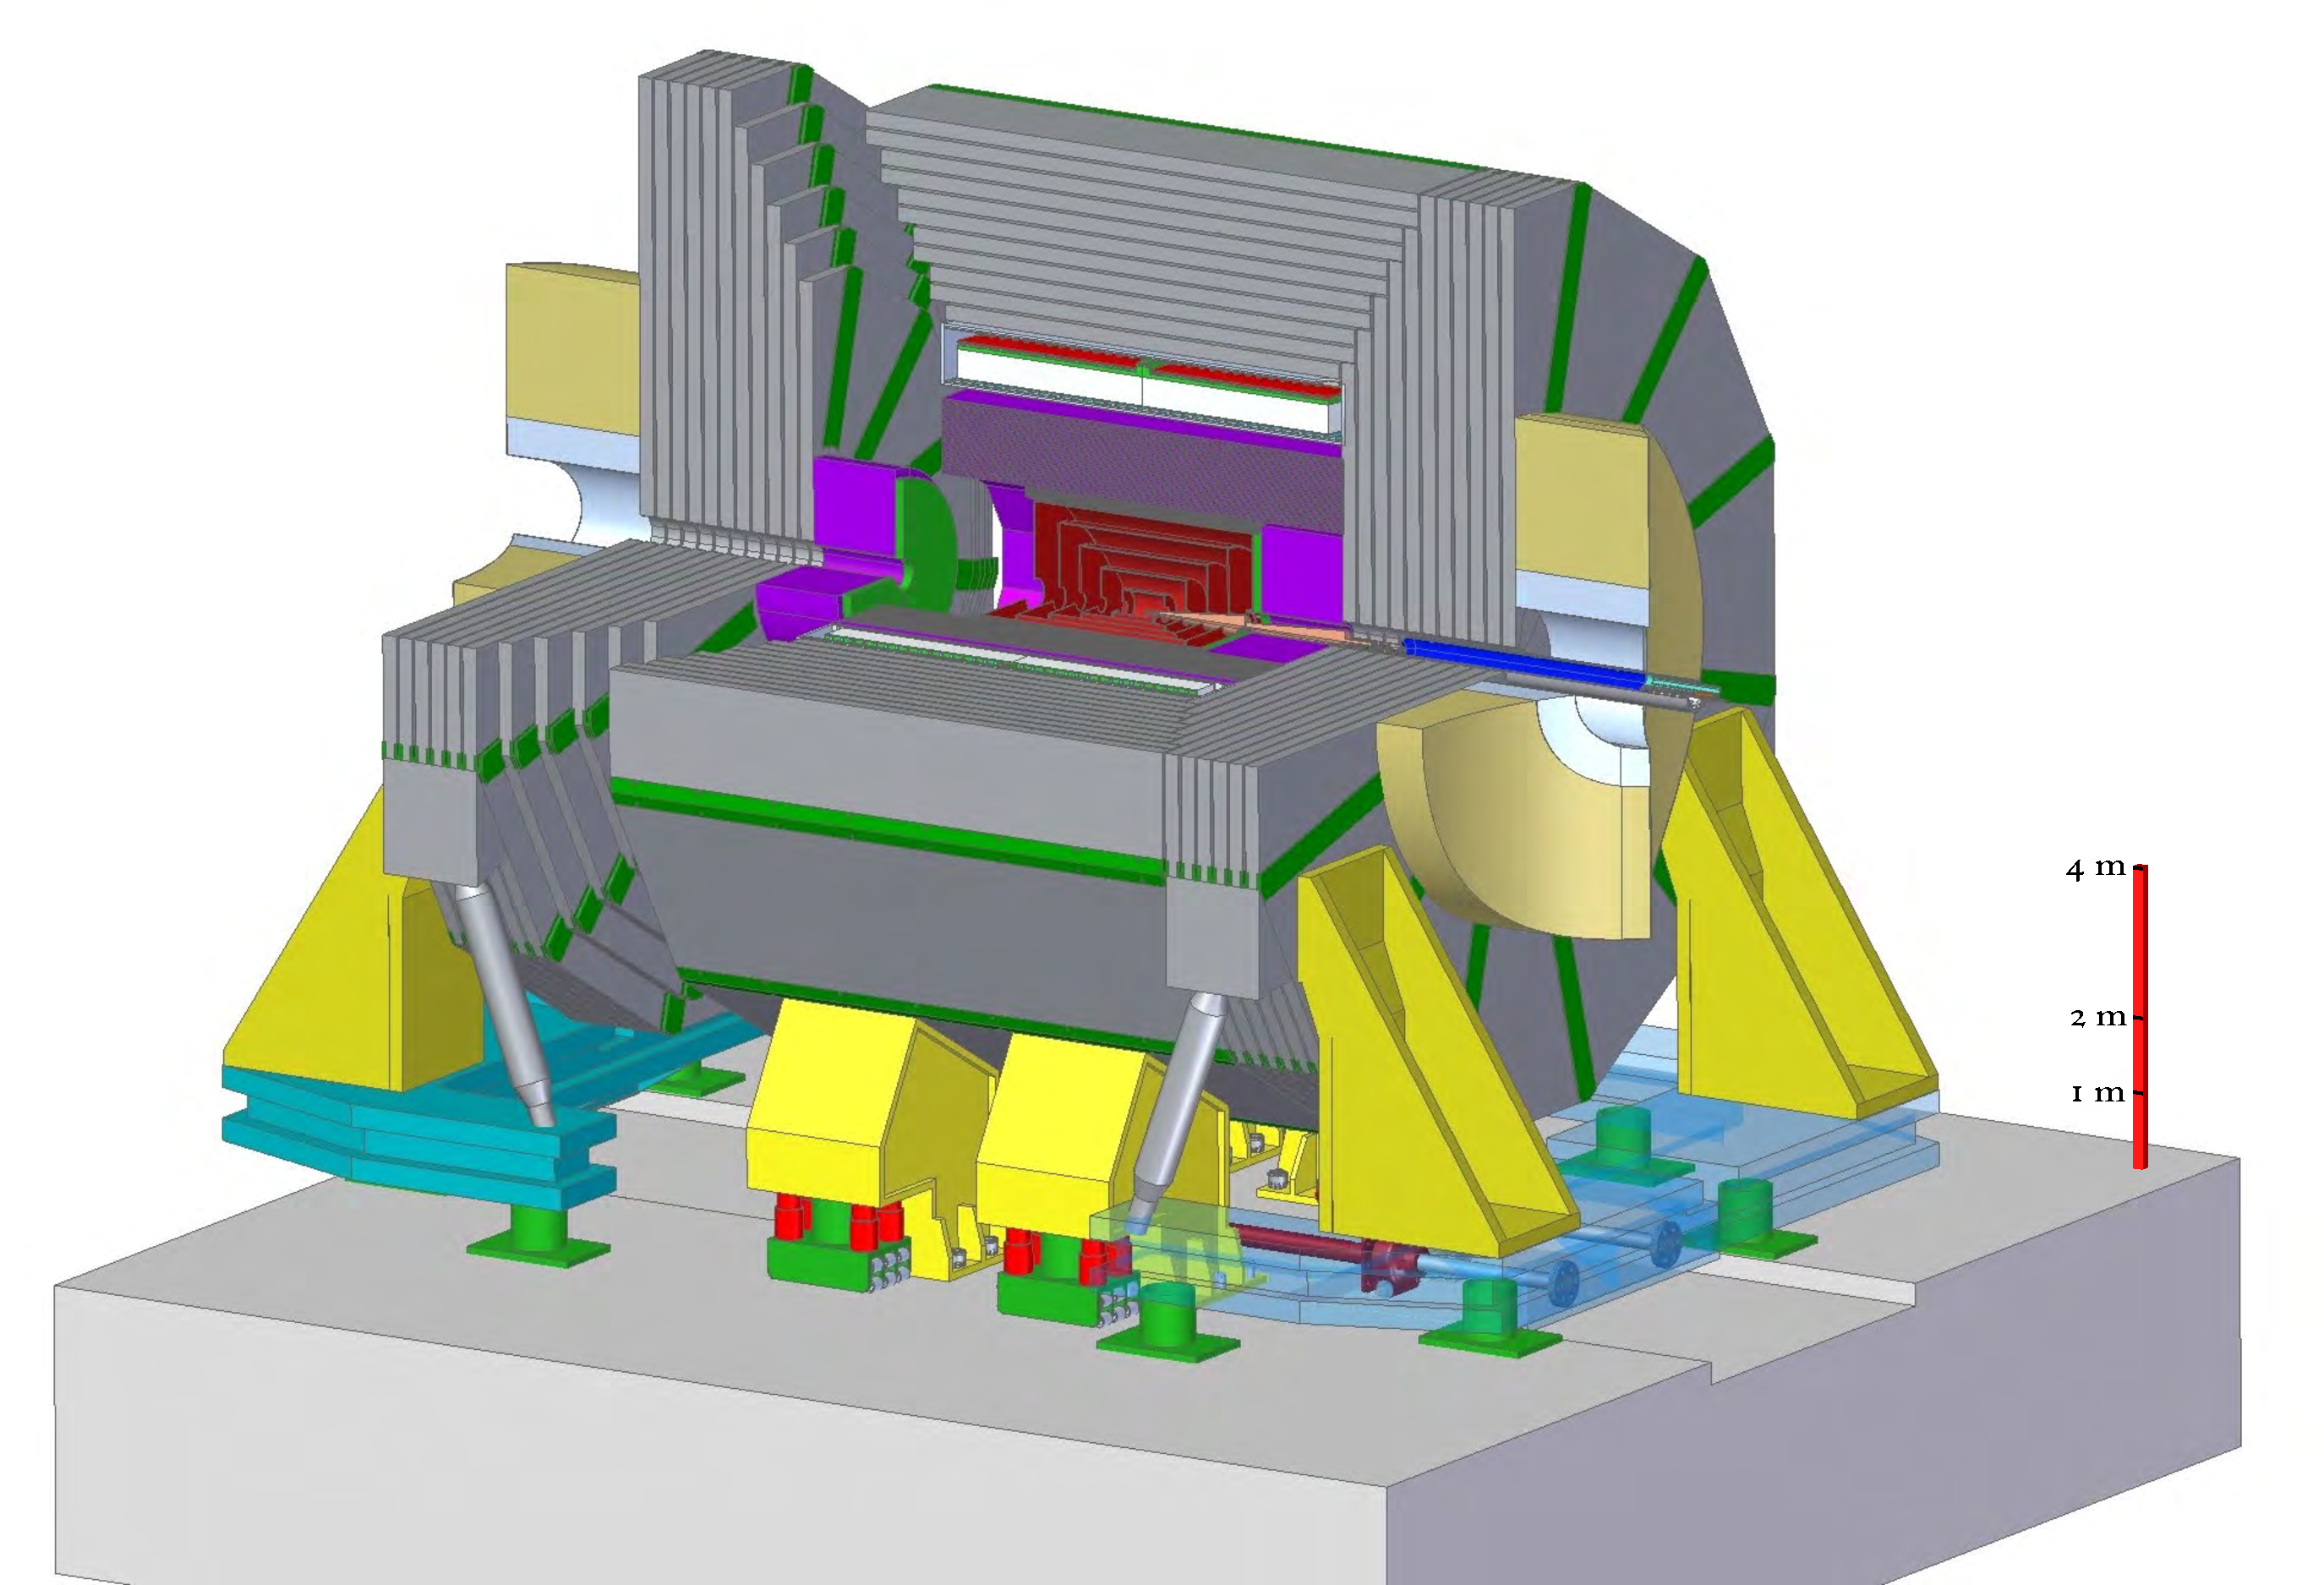
\includegraphics[width=\hsize]{figures/SiD.pdf}
\caption{The SiD detector concept.
\label{fig_sid}}
 \end{center}
 \end{figure}

Compared to the last large scale detector project in particle physics, the construction and upgrade of the LHC detectors, the emphasis for linear collider detectors is shifted towards ultimate precision. This requires \jim{detector technologies} 
with new levels of performance and minimisation of dead material in the detector, at an unprecedented level. This also requires management and control of services and, in particular, thermal management of the detector concept. Significant technological R\&D was needed to demonstrate the feasibility, and is, in fact, still ongoing, as \jim{is} discussed in the \jim{next} section.  



Over the last decade two detector concepts have emerged from the discussions in the community. Both are based on the assumption that particle flow reconstruction plays a central role in the event reconstruction. Both therefore have highly granular calorimeters, placed inside the coil which is providing the central magnetic field. Both have excellent trackers and vertexing systems. The two approaches differ in the choice of tracker technology, and in the approach taken to maximize the overall precision of the event reconstruction. ILD \jim{(\Fig{fig_ild}) } has chosen a gaseous central tracker, a time projection chamber, combined with silicon detectors inside and outside the TPC. SiD \jim{(\Fig{fig_sid}) } relies on an all silicon solution, similar to the LHC detectors, \jim{although with
much thinner silicon layers}. ILD tries to optimize the particle flow resolution by making the detector large, thus separating charged and neutral particles. SiD keeps the detector more compact, and compensates the reduced particle separation at the position of the calorimeters by using a higher central magnetic field. Both approaches have demonstrated excellent performance through prototyping and simulation, meeting or even exceeding the requirements. 

The ILC infrastructure has been designed to allow for two detectors, operated in a so-called push-pull mode. The detectors are mounted on movable platforms which can be moved relatively quickly in and out of the beam. The goal is to exchange the detectors in the IP and be ready to take data within one day. 

This baseline design with two detectors and a push-pull arrangement has distinct scientific advantages over a potential alternative of only one detector. It is also much less expensive than the previously considered alternative of having two separate interaction points with dedicated detectors. The scientific advantages arise from the complementarity of the detectors, the competition between detector teams, the opportunity for independent cross-checks of new results, and the likely larger community of participants in the scientific program. 

For both detector concepts, communities have self-organized and pre-collaborations have formed. These organizations have over the last ten years or so pushed both concepts to a remarkable level of maturity, and have, in close interaction with the different groups performing detector R\&D from around the world, demonstrated the feasibility to build and operate such high precision detectors. 

European groups have played a central role in these efforts. The ILD concept group is formed from some 70 groups from around the world, with more than half coming from Europe. The SiD collaboration has a strong basis in the Americas, but also relies on significant participation from European groups. Major contributions to the development of all sub-systems have come from Europe. Significant technological breakthroughs for example in the area of highly granular calorimeter are strongly driven by European groups. 

An important aspect of the detector concept work has been in addition to the development and demonstration of the technology the integration of the detector into the collider and into the proposed site. The location of the experiment in an earth-quake prone area poses challenges which have been addressed through R\&D on detector stability, support and service. The scheme to operate two detectors in one interaction region, the so called push-pull scheme, has no example and needed significant engineering work to demonstrate its feasibility. With strong support from particle physics laboratories in Europe, in  particular DESY and CERN, many of the most relevant questions could be answered and the feasibility of the approach could be demonstrated at least in principle. 

%%%%%%%%%%%%%%



\section{\label{sec:detectrd} Detector R\&D}


%\todo{ 1 page - Marc.}
%\todo{At present the R\&D section is copied from the original text by  Marc from Doc2. It needs to be better adapted to Doc1 and a more natural merging/transition to the detectors section. Industrial participation, interest and motivation should also be implemented.}


The capacity to reconstruct with extreme precision the characteristics of the signal states produced at the ILC is mandatory to take advantage of the inherently accurate knowledge of the scattering conditions of the beam particles. Moreover, the relatively mild running conditions allow alleviating the constraints on radiation tolerance and read-out speed. The R\&D related to each sub-system was therefore driven by a challenging and innovative trade-off to be found between very demanding resolution (granularity) and material budget requirements on the one hand, and an acceptable speed and power consumption on the other hand. Moreover, the detector steering and read-out architectures obey specific conditions: they should be operated triggerless and designed to exploit the machine duty cycle and bunch spacing to mitigate the power consumption.
In several cases, individual performances targeted by the R\&D could have been considered as nearly achieved outside of the ILC programme, but intensive R\&D was needed to realise their combination at a level well beyond previous achievements, including detailed system integration aspects. In most cases, the R\&D was aiming at an order of magnitude improvement w.r.t. the state-of-the-art. The prototyping undertaken for each experiment sub-system had as an initial goal to provide a realistic design with reliable performance and cost evaluation of the complete detector.

Overall, the R\&D on highly segmented sub-systems composing the experimental set-up was guided by the need to reconstruct each particle composing the signal states using the so-called Particle Flow Approach (PFA). The performances demonstrated by the R\&D were transferred to the Monte-Carlo description of the experiment used to predict the achievable experimental performances for each component of the physics programme.

The R\&D was conducted by a large number of groups over many years. A wide variety of technological and design options could therefore be extensively explored. Technological alternatives were investigated for all sub-systems and were compared in terms of detection performances as well as for their cost. In most cases, these detection performances were evaluated on particle beams with system aspects directly comparable to the experiment. Some beam tests were performed inside a 2 T magnetic fi�eld in order to validate the pulsed mode concept and the associated power saving.

Each calorimeter and tracking sub-system has been prototyped extensively, from small prototypes addressing all critical elements of a given sub-system up to a complete, real scale, prototype operated on beam, sometimes in combination with prototypes of other sub-systems composing the experiment. This allowed in particular to study and mature the PFA strategy with real input.

The development of tracking and vertexing devices was governed by the need of pixellated low material budget components allowing excellent momentum resolution and displaced vertices characterization, including vertex charge, with performances exceeding typically by one order of magnitude those of existing experiments.

Two alternative approaches were investigated for the main tracker, one based on a TPC and one exploiting silicon sensors, possibly pixelated. The R\&D for the TPC addressed mainly the single point resolution and ion feedback mitigation with diferent micro-pattern read-out systems (MicroMegas, GEM, ...) and showed that the performance goals can indeed be reached, with a material budget of the end-caps not exceeding 30 \% X\jim{$_0$}. The approach relying on silicon detectors concentrated on the material budget, showing that the targeted momentum resolution was reachable despite the restricted number of detector layers allowed to mitigate multiple scattering effects. These efforts have also benefited a lot from the R\&D that has been conducted for the tracker upgrades for both ATLAS and CMS, which both rely on all-silicon tracking systems. 
\jim{The tracking layers 
envisioned for the ILC are much thinner than the LHC as a consequence of the different beam conditions.}
It was also shown that, while the performance was more than adequate in terms of momentum resolution, the tracking in dense jet environments could be improved by replacing the silicon-strip sensors with a large-area pixelated tracker. 

The R\&D for the vertex detector explored the potential of several thin highly granular pixel technologies (CMOS, DEPFET, FPCCD, SoI, ...) which could off�er the projected spatial resolution and material budget. Intensive efforts were invested in read-out systems allowing to cope with the hit density induced by the beam related background, resulting in performances depending on the technology and the read-out architecture.The concept of double-sided layers was also investigated with some technologies and established up to the level of being operated near an e+e− interaction point.

A significant part of the R\&D eff�ort for the ILC detector concentrated on calorimetry, which required strategies promoting very compact and high granularity detection technologies connected to very low average power read-out micro-circuits complying with power pulsing. Major issues were addressed within the CALICE collaboration, a consortium composed of more than 300 members coming from more than 50 institutes.

The R\&D for the EM calorimeter concentrated on optimized and cost effective sensor systems, on the designs of a low power, pulsed, integrated readout electronics and an effective thermal management and calibration strategy, and on including a mechanical concept which combines large stability with minimal dead zones. A SiW based real size prototype was constructed and tested extensively on particle beams. The development of a more cost-effective technological solution, based on a scintillator and photo-multiplier matrix was also realised and some of its performances compared to those of the SiW concept.

The HCAL prototyping was governed by the need for an efficient and precise reconstruction of neutral hadron showers. Combined with stainless steel as conversion material, two read-out options were developed, one combining scintillator tiles with silicon photo-sensors read out with analog electronics, and an alternative approach based on gaseous devices (e.g. RPC) with higher segmentation but with signal encoding on one or two bits only.

The relative merits of the different ECAL and HCAL options were in particular evaluated using combined test beam campaigns providing common data which were processed with PFA software which it allowed developing and assessing at the same time. The possibility to achieve the targeted energy and topology resolutions was demonstrated even when operated in power pulsed mode.

Substantial effort was invested in developing technological solutions for the very forward calorimeters designed for robust electron and photon measurements used for integrated luminosity measurements and for bunch-to-bunch machine parameter monitoring. Satisfactory performances, including a radiation tolerance to 1 MGy, were obtained with tungsten absorber layers alternated with GaAs sensor planes read out with dedicated electronics featuring a dual gain charge amplifier providing a fast feedback for beam tuning.

%%%%%%%%%%%%%%

\section{\label{sec:soft}Software and Computing}
%\todo{ [1 page - Frank G. and Akiya
%Description of ILC software and computing requirements] }

Meeting the physics goals of the ILC programme will only be possible if the excellent detector resolution
of the two proposed ILC detector concepts described in the previous section is complemented with powerful
and sophisticated algorithms for event reconstruction and data analysis.
For over a decade the ILC community has developed and improved its software ecosystem: \emph{iLCSoft}\cite{bib:ilcsoft}, that
is based on a common event data model LCIO\cite{bib:lcio} and the generic detector description toolkit DD4hep\cite{bib:dd4hep}. 
The iLCSoft tools are used by both ILC detector concepts as well as by CLIC.
From the start a strong focus has been put on developing flexible and generic tools that can easily be applied
to other experiments or new detector concepts. This approach of developing common tools wherever possible
has helped a lot in leveraging the limited manpower and putting the focus on the algorithm development that
is crucial for the physics performance. Of particular importance here is the particle flow algorithm that aims at identifying
and reconstructing every individual particle created in the event in order to choose the best possible subdetector measurement for every particle. 
An example of individual particles reconstructed in a $t\bar t$-event is shown in \Fig{fig:ttbarevent}.
%%%%%%%%%%%%%%%%
\begin{figure}
\begin{center}
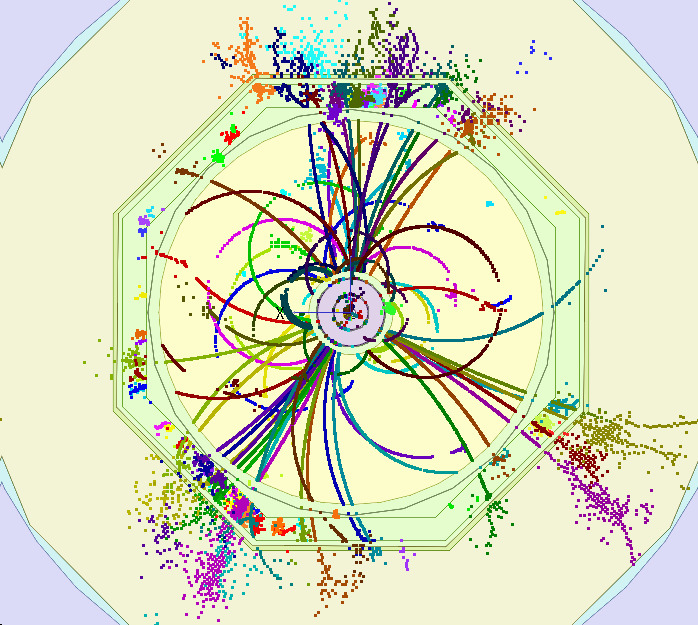
\includegraphics[width=0.95\hsize]{figures/ttbar_event_ILD.jpg}
\end{center}
\caption{Fully simulated and reconstructed $t\bar t$-event in the ILD detector, showing the individually reconstructed neutral and charged particles.}
\label{fig:ttbarevent}
\end{figure}
%%%%%%%%%%%%%%%%%%%%%%%%%%%%%%%%%%%%%%%%%%%%%%%%%%%%%%%%%%%%%%

Both detector concept groups have invested considerable effort into making their simulation models as realistic as possible.
Starting from a realistic description of the actual detector technology, dead material, gaps and imperfections have been added.
Care has been taken to include realistic services such as cables and cooling pipes, in particular in the tracking region, where
the material budget has a direct impact on the detector performance.
These simulation models have been used for large scale Monte Carlo productions and physics analyses for the TDR and more recent detector optimization
campaigns. Based on these studies, we are confident that we have a rather good and realistic understanding of the expected detector performance and physics
reach of the ILC for both detector concepts.

The development of \emph{iLCSoft} is a truly international activity, where European groups, in particular DESY and
CERN have played a leading role and should continue to do so, if the ILC will be approved. In this case
a strong focus will be on adapting the software tools for modern hardware architectures and continue to
further improve the computing and physics performance of the algorithms.


An initial computing concept for the ILC, including a first estimate of the required resources, has been developed by the LCC Software and Computing Group.
This concepts follows in general terms that of other ongoing experiments at the LHC and Belle-2 with a strong on-site computing center, complemented with large
Grid-based computing resources distributed around the world. However, due to the much lower event rates at the ILC, compared to the LHC, we will be
able to run in an un-triggered mode where collision data from every bunch crossing will be recorded. At the experiment site we require only limited computing
resources for online monitoring, QA and data buffering capabilities for a few days. Prompt reconstruction, event building and filtering of the interesting collisions
will be performed at the main ILC campus, resulting in a data reduction of around 97\%. The remainder of the data will be distributed to major participating Grid sites
in the world for further skimming and final redistribution for physics analysis.
Based on detailed physics and background simulations we estimate the total raw data rate of the ILC to be $\sim$1.5GB/s, resulting in about 10-15 PB/y storage needs.
The estimated computing power that will be needed for simulation, reconstruction and analysis will be around 200-300 kHepSpec06.
Given that these numbers are already smaller than what is needed by the LHC experiments today and an expected annual increase of 15\% and 20\% for storage and CPU
respectively at flat budget, we expect the overall computing costs for the ILC to be more than an order of magnitude smaller than those for the LHC.

\section{\label{sec:discuss}Discussion}


%\todo{ 1 page - Keisuke, Jim and Juan
%Discussion of HEP community interest and support, political progress, plan for international realization, weight on ILC250 for searches and discovery potential, opportunity for young generations, maturity of the technology -detectors and accelerator-, reliability on cost estimates, etc..}

The International Linear Collider (ILC) has a mature technical design that is ready for construction. The ILC will start as a Higgs boson factory (ILC250) where the clean operating environment, low backgrounds, adjustable beam energies and polarisations will allow model-independent measurements of the Higgs boson's absolute couplings to SM fermions and gauge bosons, most of them to better than 1\% precision, as well as determining their CP properties. The ILC250 with its high luminosity and the possibility to polarize both beams offers great opportunities to measure with high precision the couplings of the Higgs and gauge bosons. This will allow discriminating between the SM and many different BSM models; sensitivity to exotic/invisible Higgs decays adds to this discrimination. This includes  possible Dark Matter discoveries. Polarised beams will enable a versatile physics program, which is needed to test a chiral theory as the standard model and to detect the onset of new physics, in particular the electroweak couplings of right handed fermions which are largely unconstrained. Extended to higher energies in possible future upgrades, up to 500 GeV and 1 TeV, the ILC will give access to the top-quark properties including top Yukawa coupling and to the Higgs self-coupling. After reaching the top quark production threshold the ILC will become a precision top quark factory. Throughout its energy evolution  the ILC will be able to produce new BSM particles of mass up to half its centre-of-mass energy, and with sensitivity to new force particles Z' with masses ranging up to 7-12 TeV. 

A strong community of universities and laboratories world-wide is eager to realise the ILC,
to develop the detectors, and to exploit the physics opportunities.  The ILC Technical Design Report was signed by
2400 scientists from these institutions covering 48 countries and 392 Institutes/University-groups as described in Appendix \ref{Appendix1}.  This community continues to prepare for the scientific program and
will ramp up its efforts once the ILC is launched as a project.

Since no new particles beyond the SM have been discovered at the LHC, the search for new physics through high-precision studies of the Higgs boson, the top quark, and other indirect measurements with sensitivity, is urgent and compelling; this is the physics case of a linear collider. Thus a linear collider represents the best new path, complementing the high luminosity program at LHC (HL-LHC), to explore the High Energy Frontier. The ILC will measure Higgs couplings at an accuracy factor between 5-10 times better than those expected after the realisation of HL-LHC. The ILC250  being ready for construction offers in addition to its physics case a reliable project with a reasonable cost estimate similar to that of LHC, moderate time scale and well tested technologies for detectors and accelerator designs. 

The ILC’s possibility to upgrade easily to higher energies gives it a major advantage over future circular $\ee$ colliders, which have the potential to deliver higher luminosity and be more cost/power effective at energies up to around 300 GeV.~\cite{YWang2018}. 

%\todo{Idea to develop: The ILC250 if constructed in Japan, and conceived as an international global effort  should thus reinforce other programs in Asia, USA or Europe.}

%\todo{Summary of detector concepts and machine main issues. Cost in present currency. Put it in addendum. Develop more machine aspects.}

The machine R\&D during the decade leading to the ILC TDR~\cite{Behnke:2013xla} created a detailed, construction-ready design backed up by
component prototyping. The performance of the components, particularly the critical strength of the SCRF cavity gradients,
has continued to advance.  The ILC SCRF concept is even more ready for construction now.  The TDR cost for the 500 GeV collider was rescaled for ILC250~\cite{Evans:2017rvt}.
This cost estimate (based on the ILC TDR analysis) has been recently re-evaluated in Japan as shown in Appendix \ref{Appendix2}.  It has been revised for ILC250 in Japan and incorporated Japanese specific issues. The success and construction of the European X-FEL at DESY using the SCRF technology gives high reliability and confidence to the project due to the experience gained and perfect knowledge of the industrialisation process. In fact, since 2016 all linear collider conferences have included one day mini-workshops to show and promote the industrial opportunities. Very productive networking and communication has been established between industry and science. These industrial mini-workshops have been well attended with growing  interest and participation from companies and industrial associations of several key countries on the technological aspects of the project.  

Also, in preparation for the project, detector R\&D and detector concept design and optimisation has continued to be a very active
effort of the community.  The detector collaborations are prepared to broaden and expand their memberships and to move forward
with reviews of designs, including consideration of alternatives that may be proposed in the next phase of detector
optimisation before construction begins. Already, despite constrained support levels, detector R\&D has provided
the proof of principle underlying the prominent ILC detector subsystems. 
Detector prototypes fabricated and tested allow cost and full detector performance estimates. 
Furthermore, some ILC technologies and detector concepts have influenced upgrades of existing experiments.
This demonstrates the success of the ILC approaches and  provides a full size validation of ILC technological approaches.
Further studies addressing system integration are still needed. Optimization of complete experimental design, though quite advanced, also still requires additional studies. 
The few years foreseen to finalize the decision and procedure of constructing the ILC will provide the necessary 
time to make the most appropriate technological choices for each subsystem and to complete the full R\&D program in due time.

%\todo{define and refer to the interested community, TDR numbers, etc..}
%\subsection{\label{sec:discussionPol}Political situation}

On the political side, the broad interest for the ILC in Japan has been steadily growing over many years and the perspective of hosting the infrastructure in the country is being promoted by political (Diet Federation, Tohoku district) and industrial (AAA consortium) entities and finds strong support in the scientific community (KEK, HEP community, JAHEP). The project is being examined extensively within a cautious official procedure, where minimising risks of any sort is of prime importance. The Japanese MEXT's ILC Advisory Panel released its report~\cite{AdvPanel} on July 4.  This report summarises the outcomes of the several working groups (WG) that had been reviewing for several years a broad range of aspects of the ILC, including second reviews of the scientific merit and the technical design for the ILC250. 
The  Physics WG scrutinised the scientific merit of the ILC250, leading to their statement on the importance of the ILC250 to measure precisely the couplings of the Higgs boson:
\textit{If any coupling(s) is measured to be different from the Standard Model prediction, a particle-by-particle pattern of the deviation will elucidate the nature of new physics, suggesting a future direction of elementary particle physics. Mysteries in the Standard-Model such as the nature of dark matter and compositeness of the Higgs boson may also be clarified with this measurement}.
The TDR WG reviewed issues addressed in the Technical Design Report and the ILC250 design, such as cost estimate and technical feasibility.  
Other working groups of the MEXT review commented on manpower needs, organisational aspects and experience of previous large projects.
The report of the ILC Advisory Panel was followed by the beginning of deliberations in a committee and technical working group established by the Science Council of Japan (SCJ).  Another independent committee (ILC Liaison Council) led by the leadership of the majority party, the Liberal Democratic Party, has convened to encourage the national government to proceed with the ILC.

%\todo{extend this discussion with present situation on-going in Japan}

The scientific interest and political engagement of partner countries is a major concern for the Japanese authorities. Europe's expertise, capacities and involvement make it a valued potential partner. In order to address appropriately its political plurality, Europe is being approached by Japanese authorities via bilateral discussions with individual countries, where ILC may appear in a broader landscape embracing other advanced technology topics of mutual interest. Of particular interest is the collaboration of CERN, the largest European laboratory for Particle Physics. It is our current assumption that CERN will play a leading role in the European participation in the ILC along the lines of the conclusions of the 2013 Update of the European Strategy and in similar way as it has been developed for the neutrino program in USA. Given its readiness, the ILC250 is the natural bridge for the particle physics community between the LHC today and the future projects at CERN, ensuring a high level scientific program for a period after the HL-LHC. Thus  providing continuous attractive opportunities for existing talent and the incoming younger generation of bright researchers. An essential condition to maintain the vitality of the field.  Likewise, Japan seeks to secure US partnership. US Department of Energy Under Secretary of Science Paul Dabbar recently visited Japan, where he met in Tokyo with leaders promoting the ILC, and with leadership at KEK. During his visit he expressed the DOE's welcoming a decision in Japan to host the ILC, and once that happens, his interest in working in the US to find the support for US partnership on the project. Other countries like Canada, China, India, Australia, etc., are or will be be approached in the near future.

\section{\label{sec:sum}Summary \& Conclusion} 

A large world-wide community of particle physicists is eager to join the effort to build the
ILC and its detectors, and to pursue its unique physics program.  The machine technology is mature
and construction-ready. The recent construction of the European X-FEL based on SCRF technology gives high reliability to the project including its industrialisation process and cost estimation. The detector R\&D puts the detector concepts on solid footing, ready to move to finalising choices of technologies and parameters, and optimising integration. The ILC brings a natural continuity to the community after LHC and the high luminosity upgrades HL-LHC. Political actions are presently underway taken by the high level administration and political government in Japan to host the ILC in Japan. Some countries are being approached and others will follow. Physics-wise the scientific case for the ILC250 has grown stronger and will generate unique input to the effort to find the new physics and to guide the way to running at higher centre-of-mass energies.

\appendix
\part*{Appendices}
\addcontentsline{toc}{part}{Appendix}

\section{\label{Appendix1}Definition of the Community} 

Table from TDR signatories
World map high resolution indicating groups

\section{\label{Appendix2}ILC project costs} 
Tables with cost numbers: Accelerator, labour, detectors and computing

%\bibliographystyle{utphysmod}
\bibliography{ILC-ESU-refs}


\end{document}
%
% ****** End of file apssamp.tex ******
